The self-organizing map (SOM) is an unsupervised competitive learning process
developed by Teuvo Kohonen as a technique to analyze and visualize
high-dimensional data sets.  The applications of SOM are far reaching;
\cite{Kohonen2000} provides a thorough review of the SOM literature including
various applications.  SOM has been used in areas ranging from speech
recognition and image classification to breast cancer detection and gene
expression clustering.  \cite{skupin08} outline the growing interest of SOM
within geographic information science, and propose that the relationship
between SOM and GIScience should be bidirectional.  The SOM represents a
powerful method for exploring and visualizing geographic data, while GIScience
offers a wide array of tools and methods to enable the exploration of the SOM
itself.  The exploration of spatial relationships has always been of great
interest to geographers, and as Ritter states, the goal of SOM is ``to
translate \emph{data similarities} into \emph{spatial relationships}''
\cite[p. 1]{ritter99}.

The SOM is a type of artificial neural network in which neurons are
``organized'' in such a way as to project the high-dimensional relationships
of a set of training data onto a low-dimensional network structure.  The
traditional SOM uses a rectangular or hexagonal network topology
\citep{Kohonen2000}.  As shown in Figure \ref{topos} these topologies have
different properties.  In the rectangular topology, Figure \ref{topo:rook},
internal neurons are bounded by four neighbors.  In the hexagonal topology,
Figure \ref{topo:hex}, internal neurons are bounded by six neighbors. These
topologies create a well-known problem in SOM called the boundary or edge
effect.  Neurons on the boundary of the hexagonal and rectangular lattices
have fewer neighbors, which reduces their ability to interact with other
neurons during the self-organizing process.  Using a spherical lattice has
been widely suggested as a solution to the problem \citep{ritter99,
boudjemai2003, sangole03, Nishio:2006fk, wu2006}. The use of the spherical
lattice, however, does not completely overcome the boundary problem, and the
choice of which spherical topology to use for the network can be difficult to
make.

\begin{figure}
\centering
\caption{In traditional SOM either a rectangular or hexagonal topology is used.}
\subfigure[Rectangular Topology]{
  \label{topo:rook}
  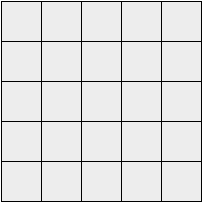
\includegraphics[width=.25\linewidth]{topo_rook.png}
}
\subfigure[Hexagonal Topology]{
  \label{topo:hex}
  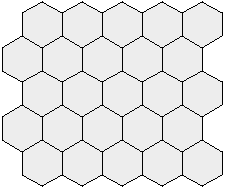
\includegraphics[width=.30\linewidth]{topo_hex.png}
}
\label{topos}
\end{figure}

Central to the ideas presented here is the concept of network regularity. A
perfectly regular network topology would be one in which every node on the
network has exactly the same number of adjacent nodes.  Any topology involving
an edge is therefore irregular.  Arranging our lattice on the surface of a
sphere seems to be an obvious way to overcome the edge.  However, there exist
only five arrangements on the sphere which are completely regular; these are
the five platonic solids \citep{ritter99, harris2000}.  Any other arrangement
of neurons on the surface of the sphere will result in an irregular topology,
as not all neurons will have the same number of neighbors.

The classic method for minimizing this irregularity is to generate the
spherical lattice by tessellating (subdividing) the sides of the icosahedron
\citep{Nishio:2006fk}.  While this method will always result in a highly
regular spherical topology, the main drawback is that the number of neurons in
the network (the network size), \(N\), grows exponentially as tessellations
are applied. In other words, one would have only very coarse control over
network size.  Other methods for arranging neurons on the sphere allow for
unlimited control over network size, but yield topologies with increased
irregularity \citep{harris2000, wu2005, Nishio:2006fk}.  To date the
literature has largely ignored the more irregular methods in favor of the
aforementioned tessellation-based methods.  A topology which yields a more
flexible network size may be desirable.  However, in order to address this
issue of network size, we must first determine the degree to which
irregularity effects the SOM.
